% !TEX program = xelatex
% Mixed raster/vector. Source: locked Jan20 2022 author PDF, pp11-14/S3/S5/S6.
% Generated viewports supply illustrations only; equations/arrows are independently checked.
\documentclass[tikz,border=2mm]{standalone}
\usepackage{fontspec,xeCJK,amsmath,amssymb,graphicx}
\setsansfont{Arial}
\setCJKmainfont[Path=/System/Library/Fonts/,BoldFont={STHeiti Medium.ttc}]{STHeiti Light.ttc}
\setCJKsansfont[Path=/System/Library/Fonts/,BoldFont={STHeiti Medium.ttc}]{STHeiti Light.ttc}
\renewcommand{\familydefault}{\sfdefault}
\usetikzlibrary{arrows.meta,calc}
\definecolor{ink}{HTML}{173646}
\definecolor{teal}{HTML}{217E80}
\definecolor{amber}{HTML}{B5712F}
\definecolor{purple}{HTML}{735098}
\definecolor{pale}{HTML}{F6F8F7}
\definecolor{warm}{HTML}{FFF6E9}
\definecolor{violet}{HTML}{F3EFF9}
\tikzset{t/.style={text=ink,font=\fontsize{16.5}{20}\selectfont,align=center,inner sep=0},
 hd/.style={t,font=\bfseries\fontsize{21}{25}\selectfont},
 sm/.style={t,font=\fontsize{15}{18}\selectfont},
 a/.style={-{Stealth[length=3mm,width=2mm]},line width=1.4pt,draw=teal,rounded corners=2pt},
 sup/.style={a,draw=amber,dashed},
 box/.style={rounded corners=4pt,line width=.8pt}}
\newcommand{\txt}[4]{\node[t,text width=#3cm]at(#1,#2){#4};}
\newcommand{\head}[4]{\node[hd,text width=#3cm]at(#1,#2){#4};}
\newcommand{\smalltxt}[4]{\node[sm,text width=#3cm]at(#1,#2){#4};}
\newcommand{\maths}[4]{\node[text=ink,font=\fontsize{#3}{#3}\selectfont,inner sep=0]at(#1,#2){\(\displaystyle #4\)};}
\newcommand{\panel}[7]{\draw[box,draw=#6!45,fill=#7](#1,#2)rectangle++(#3,#4);\pgfmathsetmacro{\pw}{#3-.3}\head{#1+#3/2}{#2+.47}{\pw}{#5}}
% Source PNG has 1536x1024 pixels and 72dpi natural size. Unmodified viewports.
\newcommand{\art}[7]{\begingroup\pgfmathsetmacro{\bt}{1024-#2-#4}\pgfmathsetmacro{\rt}{1536-#1-#3}
\node[anchor=north west,inner sep=0]at(#5,#6){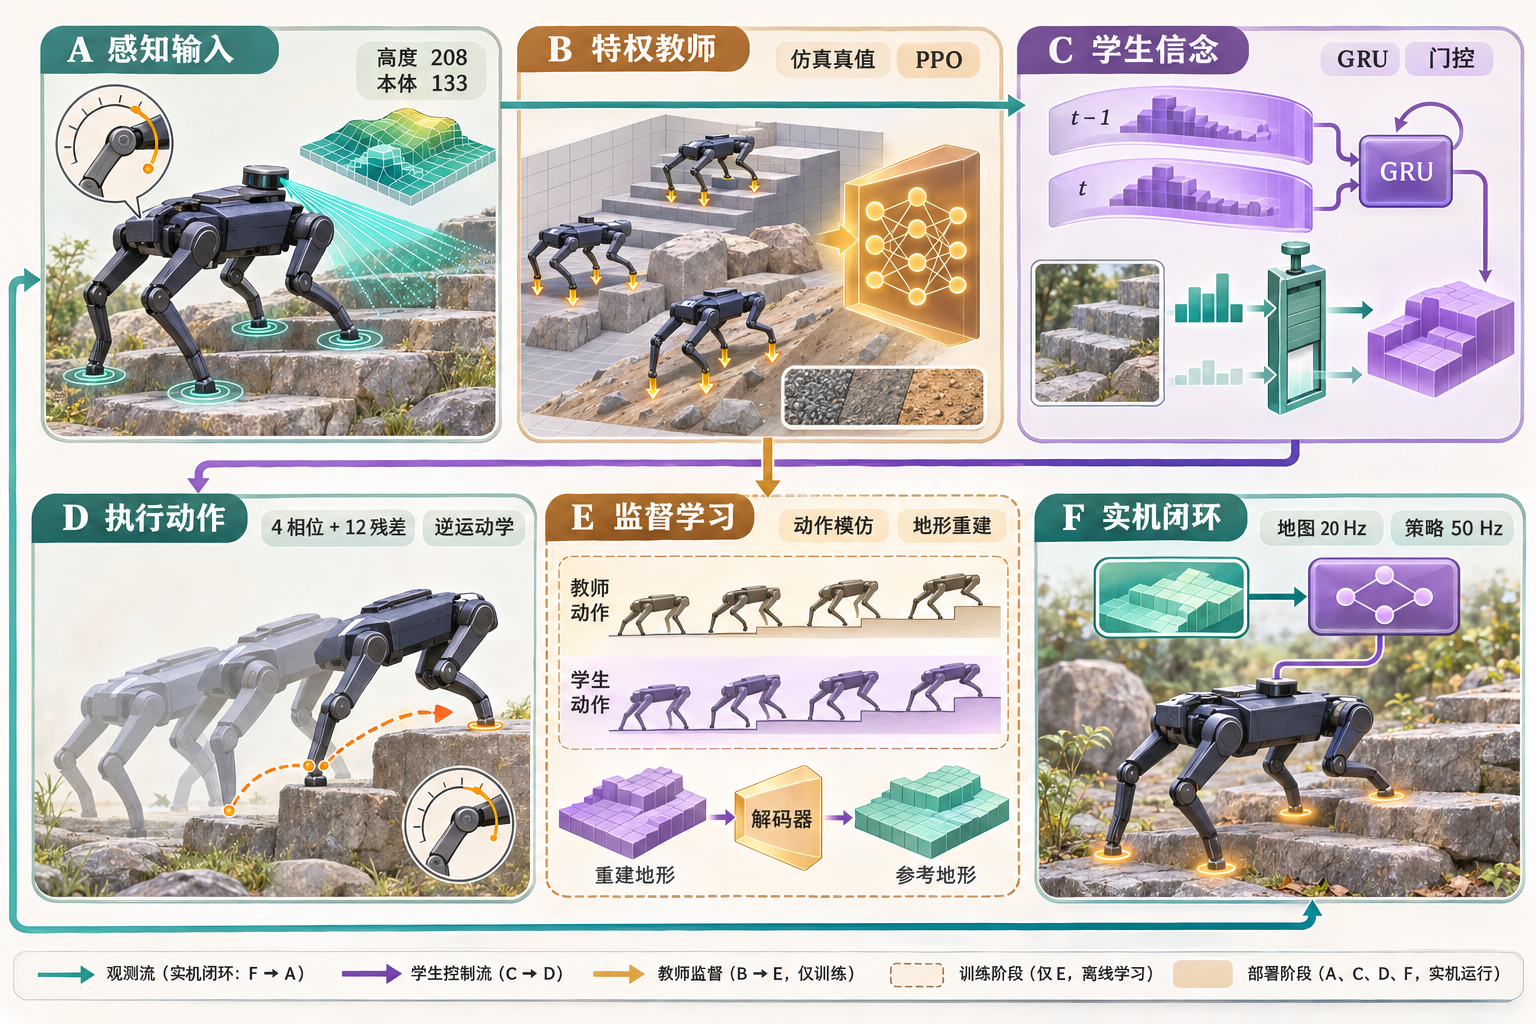
\includegraphics[trim=#1bp \bt bp \rt bp #2bp,clip,width=#7cm]{perceptive-loco-imagegen-draft.png}};\endgroup}
\begin{document}
\begin{tikzpicture}[x=1cm,y=-1cm]
\path[use as bounding box](0,0)rectangle(12.5,18.6);\fill[white](0,0)rectangle(12.5,18.6);
\head{6.25}{.5}{12}{D / F\quad 16 个动作数怎样落地？}
\art{46}{558}{482}{335}{2.55}{1.2}{7.4}
\txt{6.25}{6.8}{11.5}{策略每 20 ms 输出一次}
\maths{6.25}{7.65}{21}{a_t=[\Delta\boldsymbol\phi,\Delta\mathbf q]\in\mathbb R^{16}}
\txt{6.25}{8.6}{11.5}{四条腿各 1 个相位修正；12 个关节残差}
\draw[a](6.25,9.15)--(6.25,9.75);
\draw[box,draw=teal!40,fill=pale](.4,9.75)rectangle(12.1,13.5);
\maths{6.25}{10.5}{22}{\psi_l=\phi_l+\Delta\phi_l+\Delta\phi_0}
\txt{6.25}{11.35}{11}{名义足端轨迹 → 逆运动学}
\maths{6.25}{12.45}{21}{q^{\mathrm{target}}_{i\in l}=\mathrm{IK}[p(\psi_l)]+\Delta q_{i\in l}}
\draw[a](6.25,13.5)--(6.25,14.1);
\txt{6.25}{14.75}{11.5}{12 个关节目标角 → 机器人执行}
\txt{6.25}{15.6}{11.5}{新一帧本体感知 + 最新高程图 → 学生}
\draw[box,draw=purple!40,fill=violet](.4,16.35)rectangle(12.1,18.2);
\txt{6.25}{17.2}{11}{高程图 20 Hz，策略 50 Hz。\quad 同一张地图可被连续几次控制读取。}
\end{tikzpicture}
\end{document}
